% Part: sets-functions-relations
% Chapter: infinite
% Section: hilberts-hotel
%
\documentclass[../../../include/open-logic-section]{subfiles}

\begin{document}

\olfileid{sfr}{infinite}{hilbert}
\olsection{د هيلبرټ هوټل}

د طبيعي عددونو سټ په څرګند ډول نامتناهي دے۔ نو که نۀ غواړو طبيعي
عددونه له مخکښې \emph{ومنـو}، زموږ لومړے ګام بايد دا وي چې نامتناهي
سټ په داسې اصطلاحاتو کښې وپېژنو چې خپله د طبيعي عددونو يادولو ته
اړتيا ونۀ لري۔ دا يوه ښۀ لار ده چې هيلبرټ په 1924 کال کښې په يوه
وينا کښې وړاندې کړه۔ هغه غواړي چې داسې تصور وکړو:
\begin{quote}
[\ldots] يو هوټل چې متناهي شمېر کوټې لري۔ په دې هره کوټه کښې دې
کټ مټ يو مېلمه اوسېږي۔ که مېلمانه اوس خپلې کوټې په کوم ډول سره
بدلې کړي، [خو] داسې چې په هره کوټه کښې بيا هم تر يوه زيات کس نۀ
وي، نو هېڅ کوټه به خالي نشي، او د هوټل خاوند په دې توګه د نوي
رارسېدونکي مېلمه دپاره نوے ځاے نشي پيدا کولے [\ldots
\textparagraph \ldots]

اوس ټاکو چې هوټل به نامتناهي ډېرې شمېرل شوې کوټې $1$، $2$، $3$،
$4$، $5$، \dots ولري او په هره کښې کټ مټ يو مېلمه وي۔ کله چې يو
نوے مېلمه راشي، خاوند ته يوازې دا پکار دي چې هر پخوانے مېلمه هغې
کوټې ته ولېږي چې شمېر ئې يو زيات وي؛ بيا کوټه~$1$ د نوي رارسېدونکي
مېلمه دپاره خالي کېږي۔
	\begin{center}
		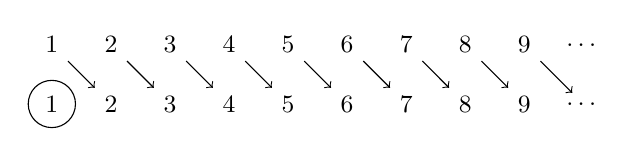
\begin{tikzpicture}[scale = .75]
		\foreach \x in {1, 2, 3, 4, 5, 6, 7, 8, 9}
		{
			\node (\x a) at (\x, 1) {\small{\x}};
			\node (\x b) at (\x, 2) {\small{\x}};
		}
		\node (dotsa) at (10, 1) {\small{\ldots}};
		\node (dotsb) at (10, 2) {\small{\ldots}};
		\draw[->] (1b)--(2a);
		\draw[->] (2b)--(3a);
		\draw[->] (3b)--(4a);
		\draw[->] (4b)--(5a);
		\draw[->] (5b)--(6a);
		\draw[->] (6b)--(7a);
		\draw[->] (7b)--(8a);
		\draw[->] (8b)--(9a);
		\draw[->] (9b)--(dotsa);
		\draw (1,1) circle (.4);
		\end{tikzpicture}
	\end{center}
	(په \citealt[730]{EwaldSieg2013} کښې خپور شوے؛ ژباړه زموږ ده)
\end{quote}
مهم ټکی دا دے چې د هيلبرټ هوټل نامتناهي ډېرې کوټې لري؛ او د هغه
تشريح د دې خبرې تعريف ګڼلے شو چې دا څه معنا لري۔ په رښتيا، د
ډېډېکېنډ لار همدا وه (البته دلته په لوے زماني بې‌ځايه‌والي سره
وړاندې شوې؛ د ډېډېکېنډ تعريف د \citeyear{Dedekind1888} کال دے):

\begin{defn}\ollabel{defn:DedekindInfinite}
يو سټ $A$ هله او يوازې هله \emph{د ډېډېکېنډ له مخې نامتناهي} دے
چې له~$A$ څخه د~$A$ يو حقيقي فرعي سټ ته کومه !!a{injection} موجوده
وي۔ يعنې داسې $o \in A$ او !!a{injection} $f \colon A \to A$ شته
چې $o \notin \ran{f}$ وي۔
\end{defn}

\end{document}
